\documentclass{article}

\usepackage{fancyhdr} % Required for custom headers
\usepackage{lastpage} % Required to determine the last page for the footer
\usepackage{amsmath}
\usepackage{amsfonts}
\usepackage{graphicx}
\usepackage{subfigure}
\usepackage{listings}
\usepackage{booktabs}
\usepackage[hidelinks]{hyperref}
% \usepackage{epstopdf} uncomment this line if using MiKTeX

% Margins
\topmargin=-0.45in
\evensidemargin=0in
\oddsidemargin=0in
\textwidth=6.5in
\textheight=9.0in
\headsep=0.25in

\linespread{1.25} % Line spacing

% Set up the header and footer
\pagestyle{fancy}
\lhead{\authorName} % Top left header
\chead{\classID\ \hwTitle} % Top center header
\rhead{\studentID} % Top right header
\lfoot{} % Bottom left footer
\cfoot{} % Bottom center footer
\rfoot{Page\ \thepage\ of~\pageref{LastPage}} % Bottom right footer
\renewcommand{\headrulewidth}{0.4pt} % Size of the header rule
\renewcommand{\footrulewidth}{0.4pt} % Size of the footer rule

\setlength{\parindent}{0pt} % Removes all indentation from paragraphs

\setcounter{secnumdepth}{0} % Removes default section numbers
\newcounter{problemCounter} % Creates a counter to keep track of the number of problems

\newcommand{\problemName}{}
\newenvironment{problem}[1][Problem \arabic{problemCounter}]{
	\stepcounter{problemCounter} % Increase counter for number of problems
	\renewcommand{\problemName}{#1} % Assign \problemName the name of the problem
	\section{\problemName} % Make a section in the document with the custom problem count
}{}

\newcommand{\subproblemName}{}
	\newenvironment{subproblem}[1]{
	\renewcommand{\subproblemName}{#1} % Assign \subproblemName to the name of the section from the environment argument
	\subsection{\subproblemName} % Make a subsection with the custom name of the subsection
}{}

%----------------------------------------------------------------------------------------
%	MATH OPERATOR
%----------------------------------------------------------------------------------------

\DeclareMathOperator*{\argmin}{arg\,min}
\DeclareMathOperator*{\argmax}{arg\,max}

%----------------------------------------------------------------------------------------
%	NAME AND CLASS SECTION
%----------------------------------------------------------------------------------------

\newcommand{\hwTitle}{Assignment\ \#3} % Assignment title
\newcommand{\dueDate}{Thursday,\ April\ 7,\ 2016} % Due date
\newcommand{\classID}{ENGG\ 5202} % Course/Class
\newcommand{\authorName}{Kai Chen} % Your name
\newcommand{\studentID}{1155070509} % Your student ID

%----------------------------------------------------------------------------------------
%	TITLE PAGE
%----------------------------------------------------------------------------------------

\title{
	\vspace{2in}
	\textmd{\textbf{\classID:\ \hwTitle}}\\
	\normalsize\vspace{0.1in}\small{Due\ on\ \dueDate}
	\vspace{3in}
}

\author{\textbf{\authorName}}
\date{} % Insert date here if you want it to appear below your name

%----------------------------------------------------------------------------------------

\begin{document}
\maketitle
\setcounter{page}{0}
\thispagestyle{empty}
\newpage

%----------------------------------------------------------------------------------------
%	PROBLEM 1
%----------------------------------------------------------------------------------------

% To have just one problem per page, simply put a \clearpage after each problem

\begin{problem}

\begin{subproblem}{1.1}
\begin{align*}
K_3(x, x') &= K_1(x, x') + K_2(x, x') \\
&= \Phi_1(x)\Phi_1(x') + \Phi_2(x)\Phi_2(x') \\
&= [\Phi_1(x), \Phi_2(x)]\cdot[\Phi_1(x'), \Phi_2(x')] \\
\Phi_3(x) &= [\Phi_1(x), \Phi_2(x)]
\end{align*}
\end{subproblem}

\begin{subproblem}{1.2}
\begin{align*}
K_3(x, x') &= K_1(x, x')K_2(x, x') \\
&= \Phi_1(x)\Phi_1(x')\Phi_2(x)\Phi_2(x') \\
\Phi_3(x) &= \Phi_1(x)\Phi_2(x)
\end{align*}
\end{subproblem}

\begin{subproblem}{1.3}
\begin{align*}
K(x, x') &= 1 + x \cdot x' + 4{(x \cdot x')}^2 \\
&= 1 + x_1x_1' + x_2x_2' + 4{(x_1x_1' + x_2x_2')}^2 \\
&= 1 + x_1x_1' + x_2x_2' + 4x_1^2x_1'^2 + 4x_2^2x_2'^2 + 8x_1x_1'x_2x_2' \\
\Phi(x) &= [1\ x_1\ x_2\ 2x_1^2\ 2x_2^2\ 2\sqrt{2}x_1x_2]
\end{align*}
\end{subproblem}

\end{problem}

%----------------------------------------------------------------------------------------
%	PROBLEM 2
%----------------------------------------------------------------------------------------

\begin{problem}

\begin{subproblem}{2.1}
The best kernels and corresponding test errors for different datasets are shown in Table~\ref{tab:2_1}. Support vectors are plotted in Figure~\ref{fig:2_1} to Figure~\ref{fig:2_3}.
\begin{table}[htbp]
\centering
\caption{Choosing kernel for different datasets}\label{tab:2_1}
\begin{tabular}{ccc}
\toprule
Dataset & Best kernel & Test error \\
\midrule
Set1 & Linear kernel & 4.46\% \\
Set2 & Radial basis kernel & 1.4\% \\
Set3 & Radial basis kernel & 0\% \\
\bottomrule
\end{tabular}
\end{table}

\begin{figure}[htbp]
\centering
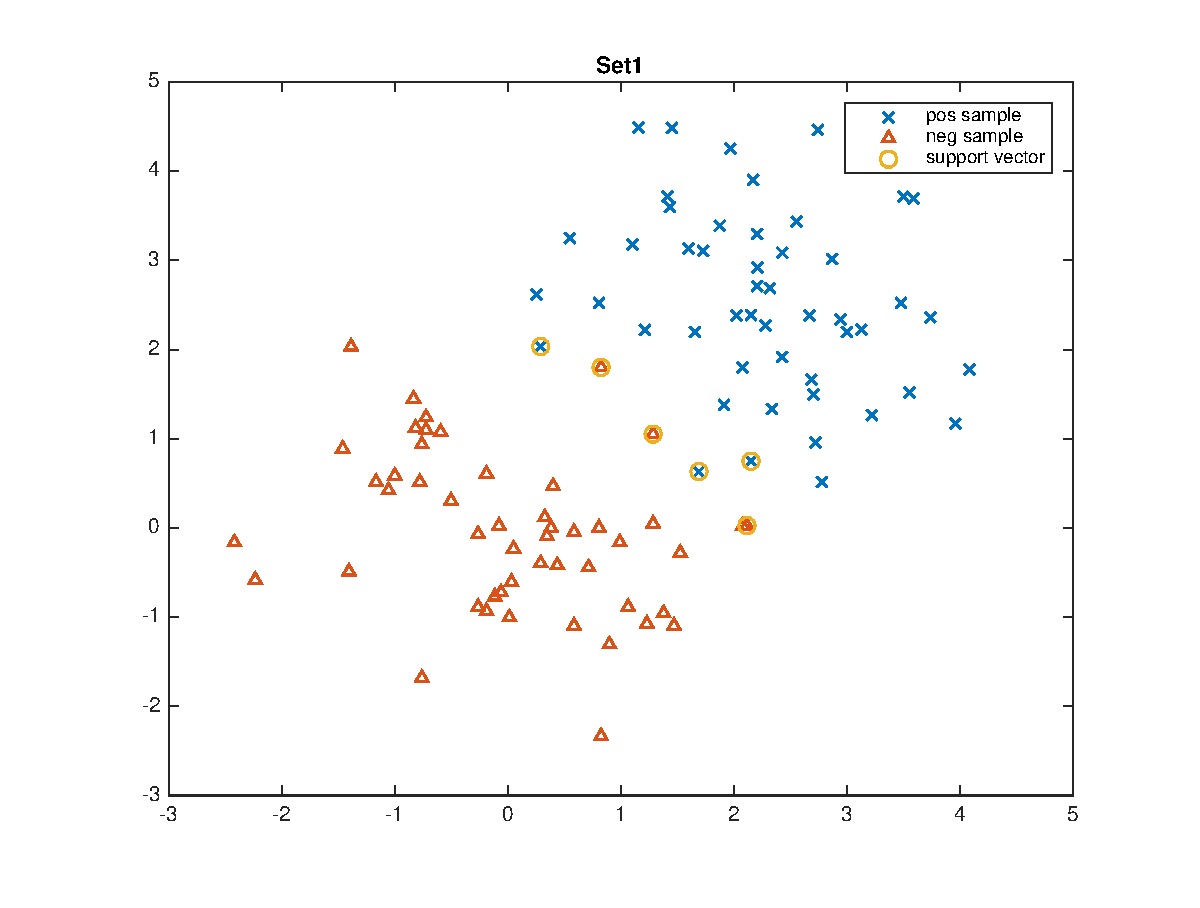
\includegraphics[width=4in]{image/2_1}
\caption{Support vectors of Set1}\label{fig:2_1}
\end{figure}

\begin{figure}[htbp]
\centering
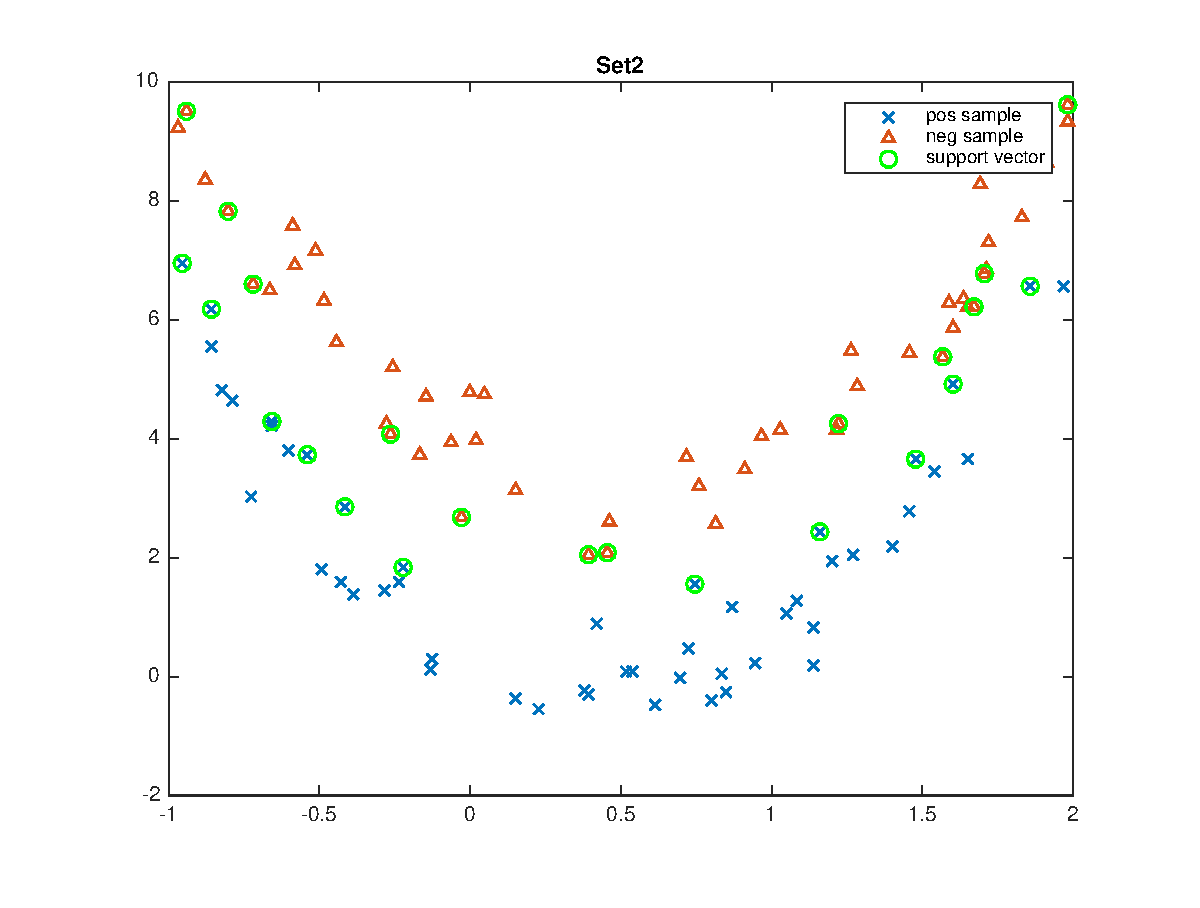
\includegraphics[width=4in]{image/2_2}
\caption{Support vectors of Set2}\label{fig:2_2}
\end{figure}

\begin{figure}[htbp]
\centering
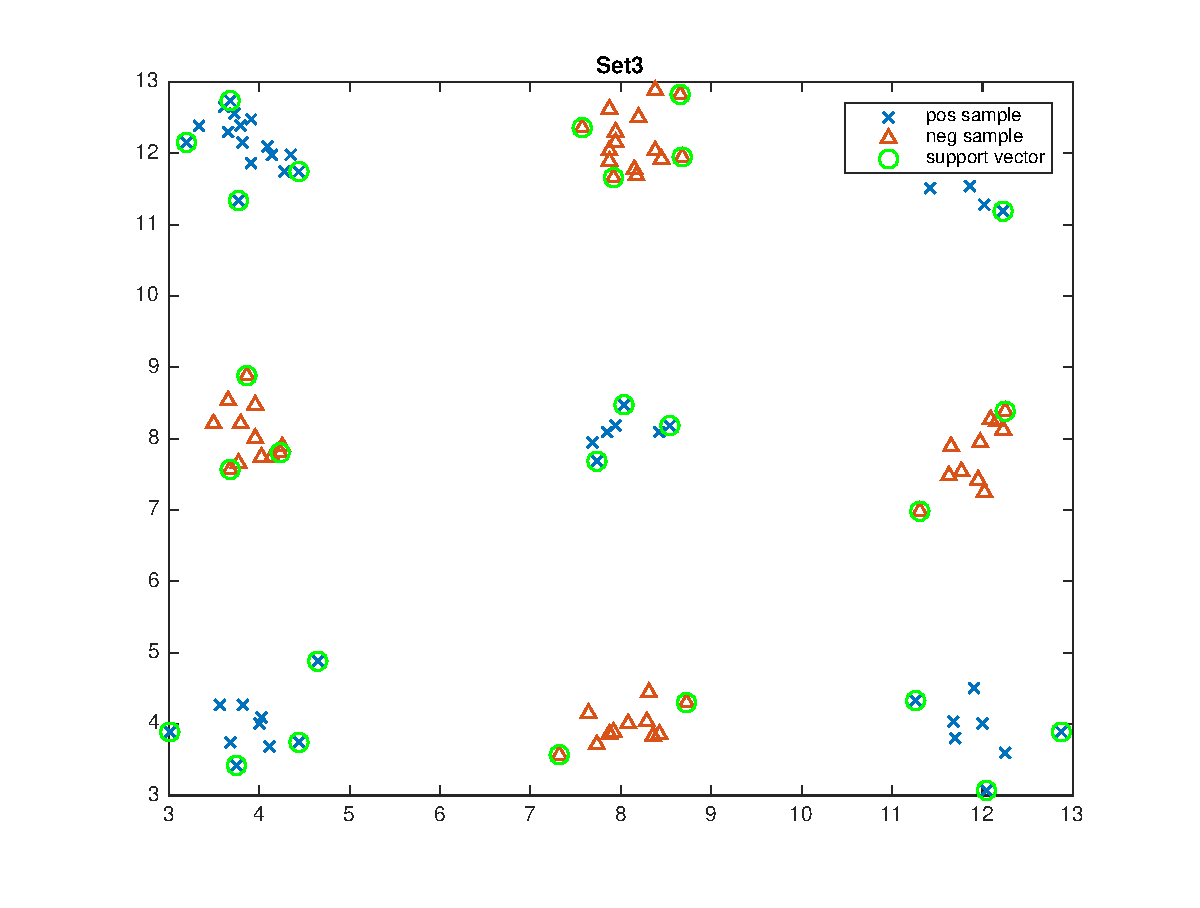
\includegraphics[width=4in]{image/2_3}
\caption{Support vectors of Set3}\label{fig:2_3}
\end{figure}
\end{subproblem}

\begin{subproblem}{2.2}
Test errors are shown in Table~\ref{tab:2_2}.
\begin{table}[htbp]
\centering
\caption{SVM classification error of different kernels}\label{tab:2_2}
\begin{tabular}{cc}
\toprule
Kernel & Test error \\
\midrule
Linear kernel & 13.75\% \\
Polynomial kernel & 12\% \\
Radial basis kernel & 8.5\% \\
\bottomrule
\end{tabular}
\end{table}
\end{subproblem}

\end{problem}

%----------------------------------------------------------------------------------------
%	PROBLEM 3
%----------------------------------------------------------------------------------------

\begin{problem}

\begin{subproblem}{3.1}
The dicision boundary is shown in Figure~\ref{fig:3_1}.
\begin{figure}[htbp]
\centering
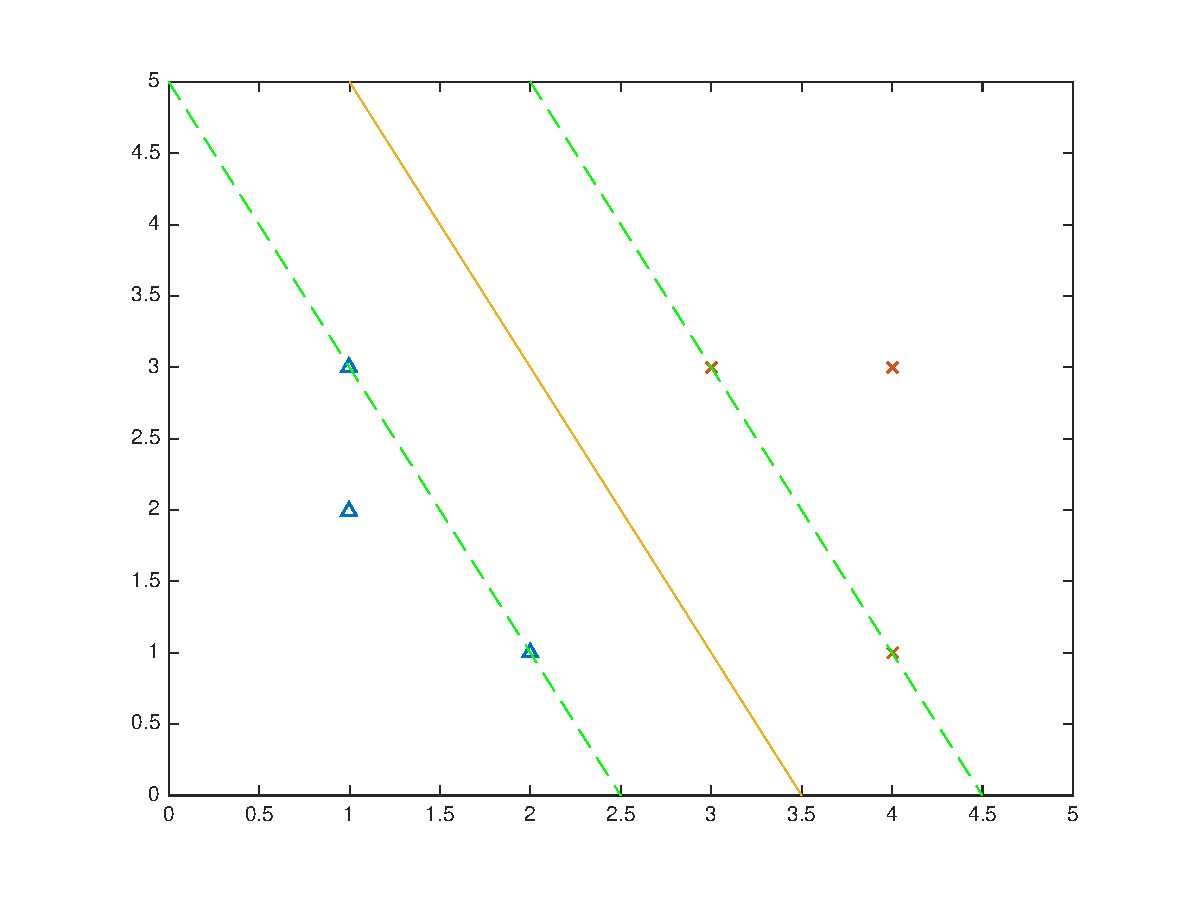
\includegraphics[width=4in]{image/3_1}
\caption{SVM classifier}\label{fig:3_1}
\end{figure}
\end{subproblem}

\begin{subproblem}{3.2}
Support vectors are these 4 points: \\
(1, 3) \\
(2, 1) \\
(3, 3) \\
(4, 1)
\end{subproblem}

\begin{subproblem}{3.3}
Yes, for example, if a negative sample (3, 1) is added, then the number of support vectors will be decreased to 3.
\end{subproblem}

\begin{subproblem}{3.4}
The leave-one-out cross-validation error is 
\end{subproblem}

\end{problem}

%----------------------------------------------------------------------------------------
%	PROBLEM 4
%----------------------------------------------------------------------------------------

\begin{problem}

\begin{subproblem}{4.1}
The disicion boundary of the first decision stump chosen by Adaboost is drawn in Figure~\ref{fig:4_1}.
\begin{figure}[htbp]
\centering
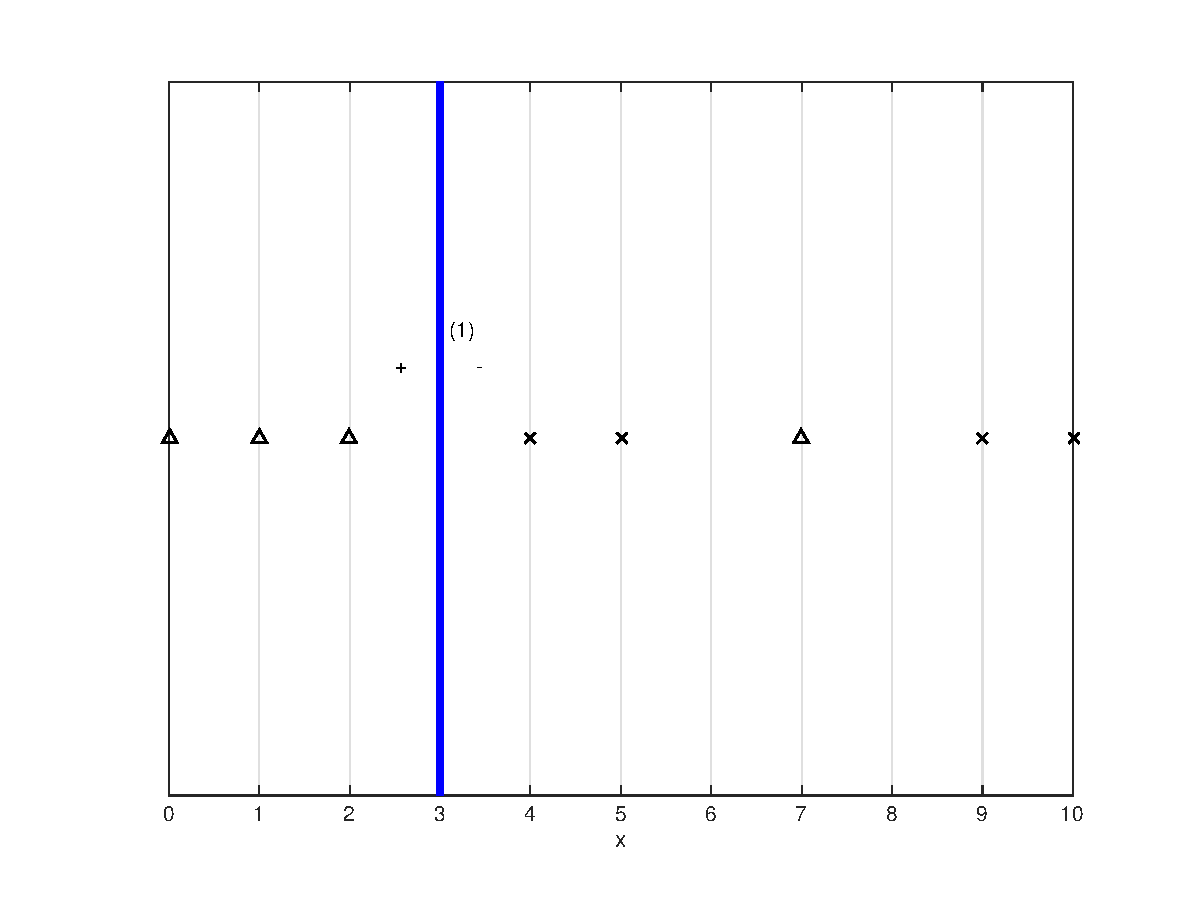
\includegraphics[width=4in]{image/4_1}
\caption{Decision boundary of the first decision stump}\label{fig:4_1}
\end{figure}
\end{subproblem}

\begin{subproblem}{4.2}
Calculate the vote of the first classifier
\begin{align*}
\epsilon_1 &= 0.5 - \frac{1}{2}(\sum_{i=1}^n\tilde{W}_i^{(0)}y_i h(x_i;\hat{\theta}_1)) \\ 
&= \frac{1}{8} \\
\alpha_1 &= 0.5\ln\frac{1-\epsilon_1}{\epsilon_1} \\
&= 0.5\ln7
\end{align*}
The sixth sample is misclassified, so
\begin{align*}
W_6^{(1)} &= W_6^{(0)}\cdot\exp \{-y_6\alpha_1h(x_6;\hat{\theta}_1)\} = \frac{7}{8}\sqrt{e} \\
W_i^{(1)} &= W_i^{(0)} = \frac{1}{8} \mathrm{\quad for\ all\ } i \neq 6
\end{align*}
So we can get the new weight for all training samples
\begin{align*}
\tilde{W}_6^{(1)} &\approx 0.6225 \\
\tilde{W}_i^{(1)} &\approx 0.0539 \mathrm{\quad for\ all\ } i \neq 6
\end{align*}
Through line search, we can get the decision boundary of the second decision stump, as is shown in Figure~\ref{fig:4_2}.
\begin{figure}[htbp]
\centering
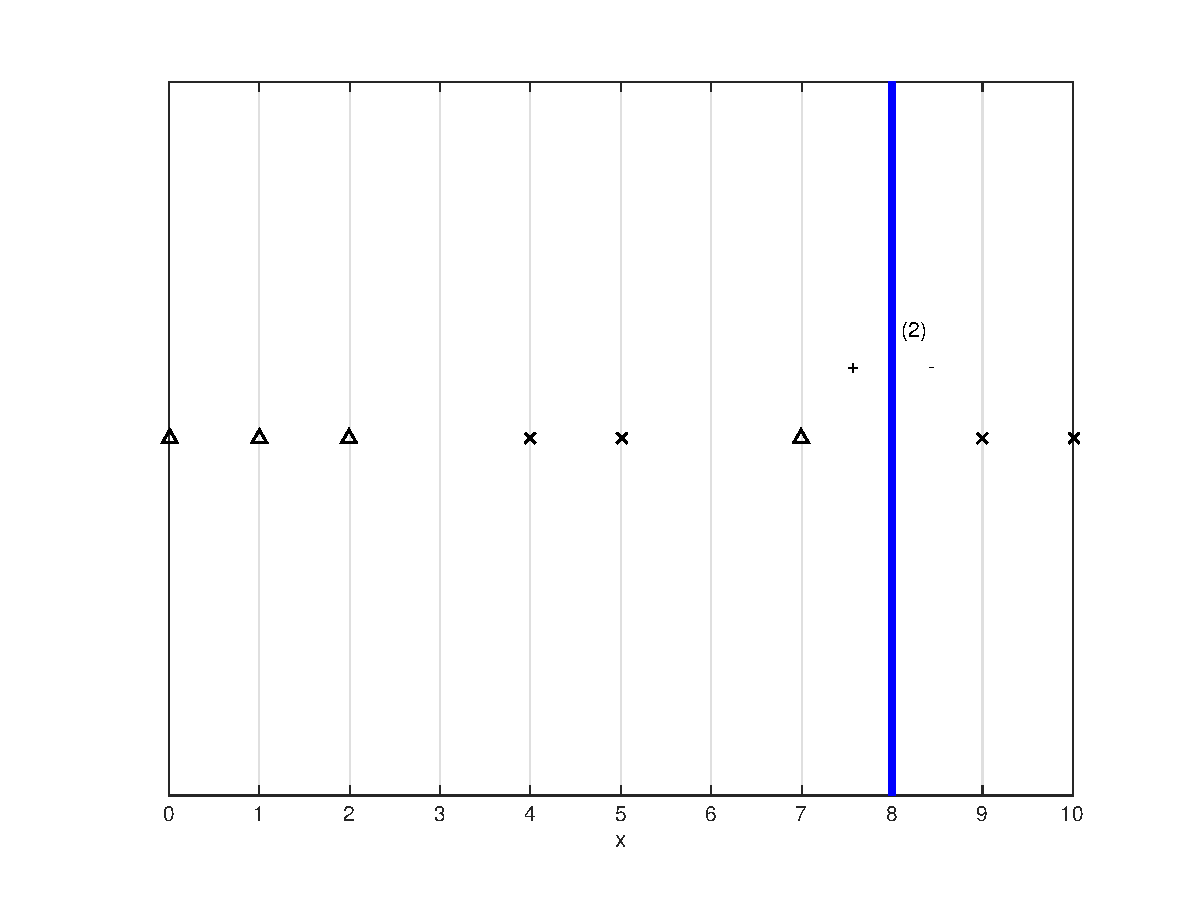
\includegraphics[width=4in]{image/4_2}
\caption{Decision boundary of the second decision stump}\label{fig:4_2}
\end{figure}
\end{subproblem}

\begin{subproblem}{4.3}
The decision boundary of the first decision stump chosen by Adaboost is drawn in Figure~\ref{fig:4_3}.
\begin{figure}[htbp]
\centering
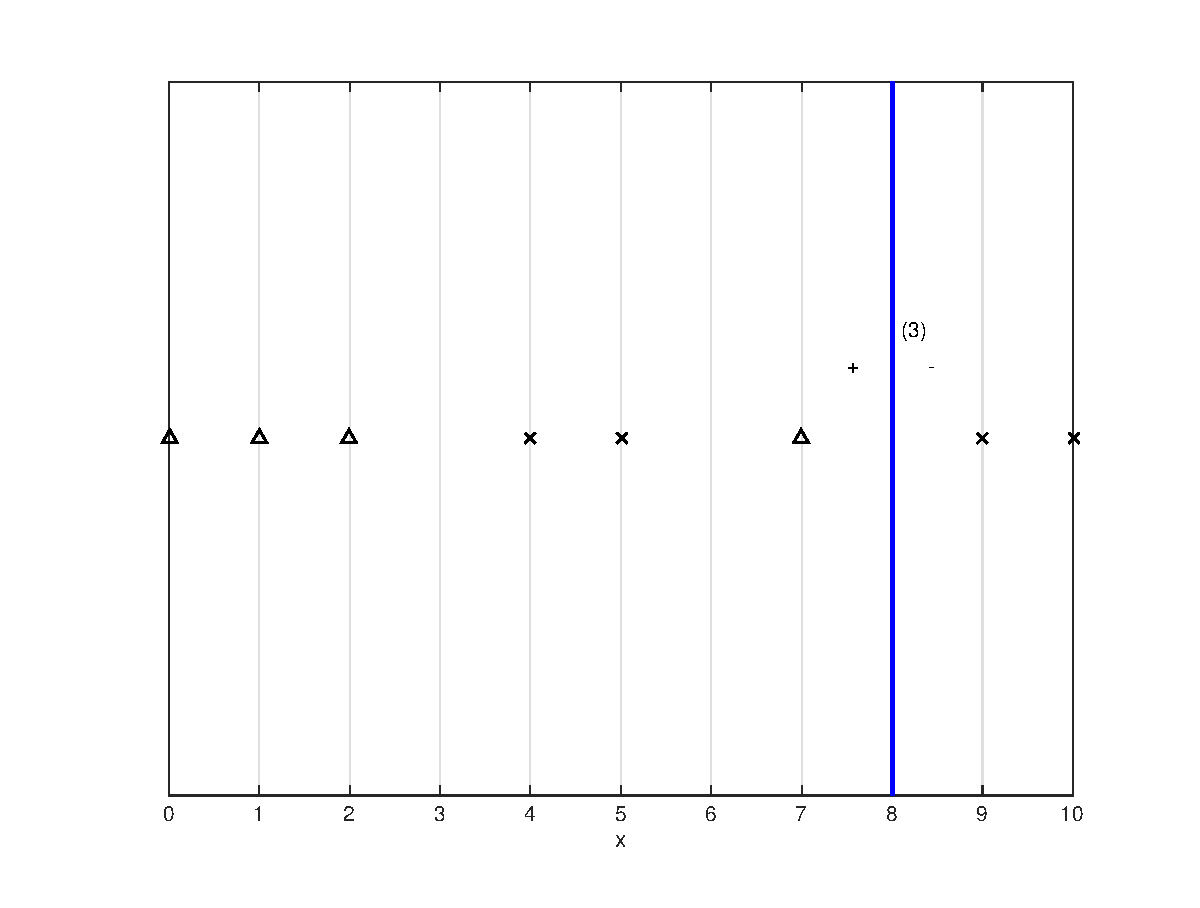
\includegraphics[width=4in]{image/4_3}
\caption{Decision boundary of the first decision stump}\label{fig:4_3}
\end{figure}
\end{subproblem}

\begin{subproblem}{4.4}
The two finally trained classifiers will behave similarly.
\end{subproblem}

\begin{subproblem}{4.5}

\end{subproblem}

\end{problem}

\end{document}
